\famichapter{Data Management and Data Model}{This chapter documents the MongoDB
data model: the thirteen entities, their relationships, and the constraints and
indexes that protect data integrity.}{ch:data}

\section{Database Design}

FamiPet uses MongoDB~\cite{mongodb} as its primary store. The schema is defined
in thirteen Mongoose~\cite{mongoose} models, all located in \texttt{backend/models/}. Figure~\ref{fig:er}
shows the entity--relationship view of the store. Dashed lines mark references
whose target documents are populated through Mongoose \texttt{populate}.

\begin{figure}[p]
    \centering
    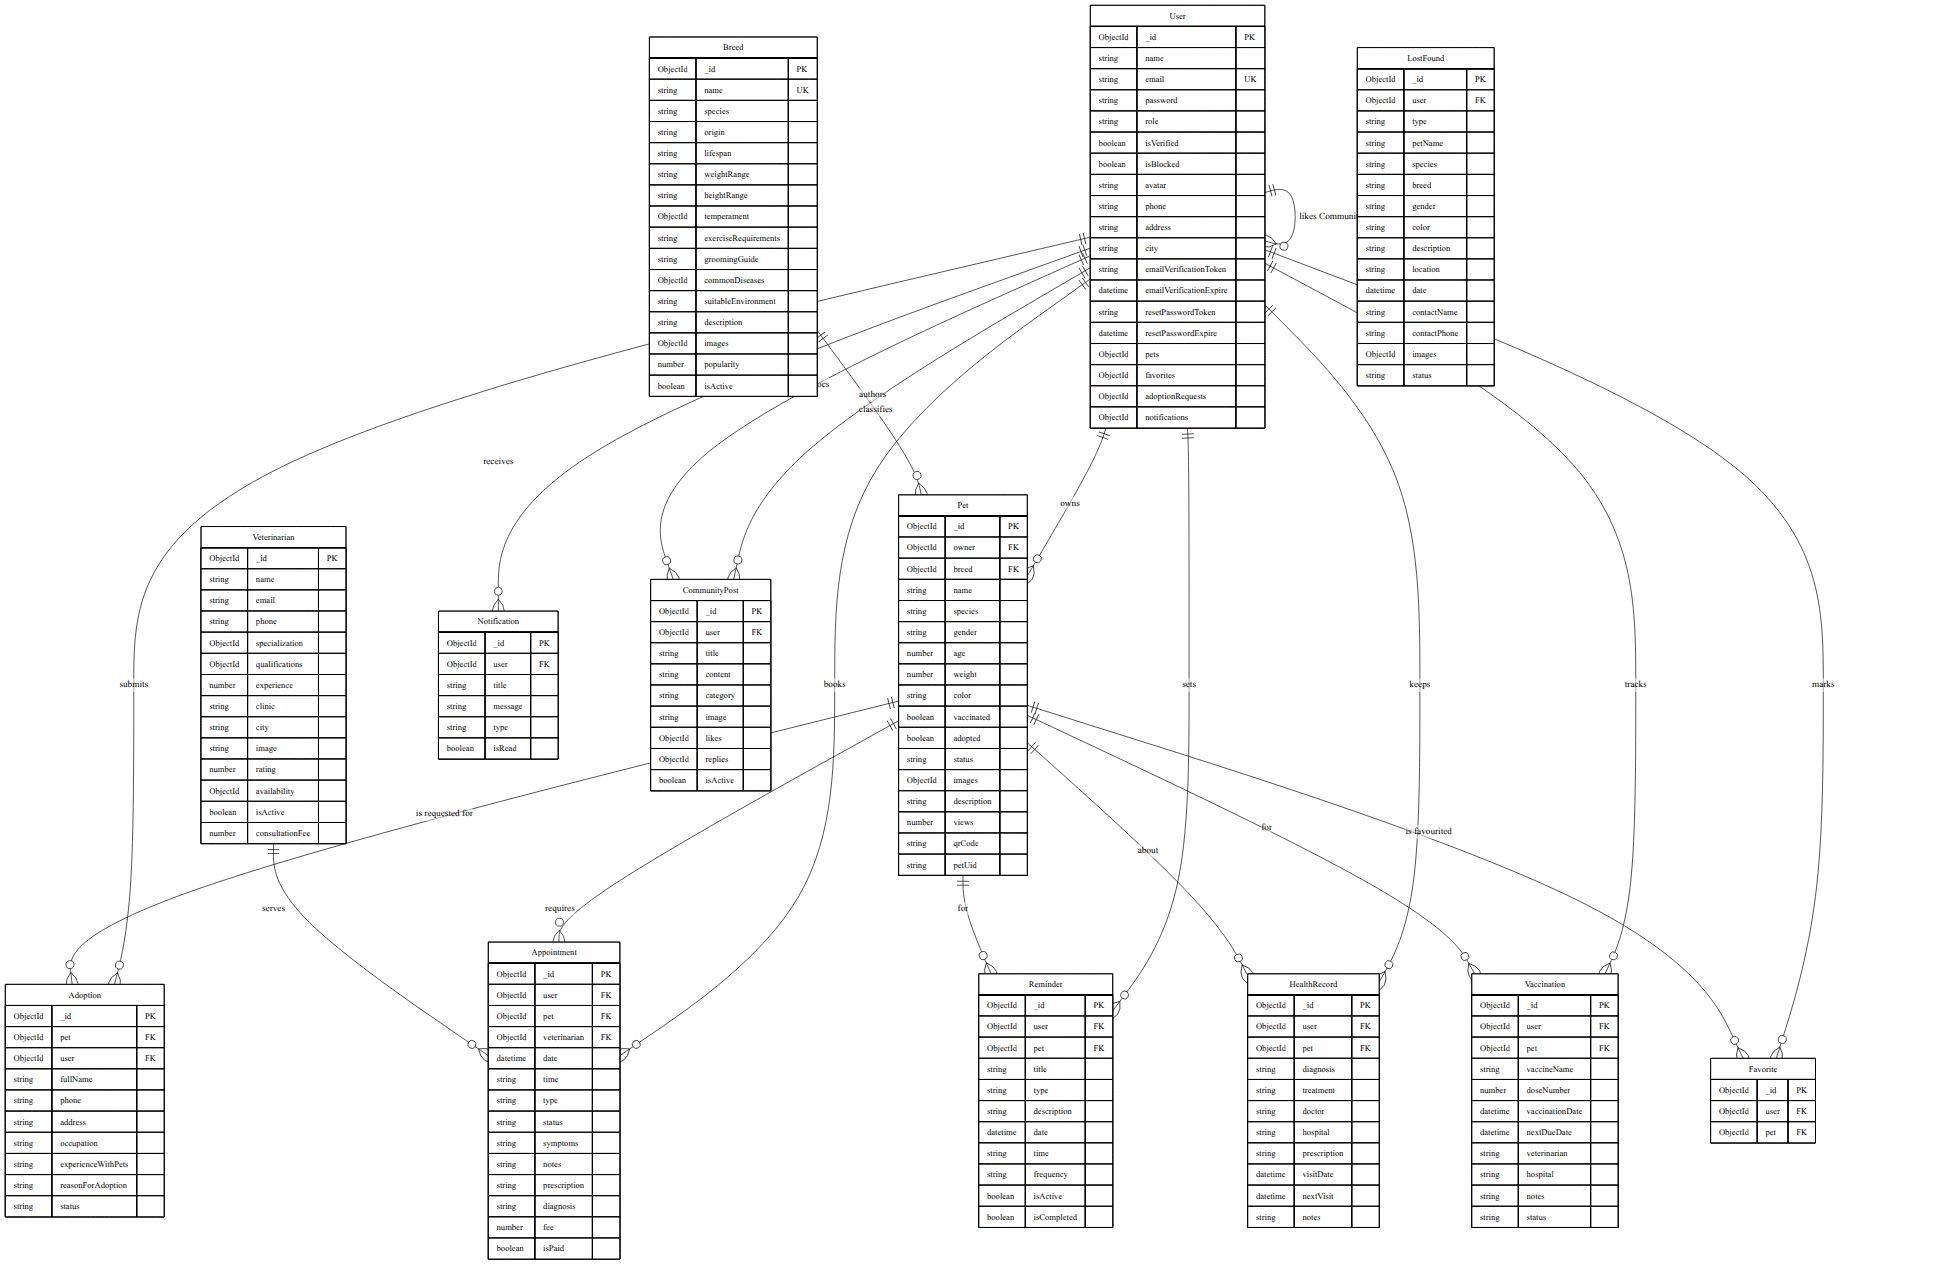
\includegraphics[width=\textwidth]{figures/08-er-diagram.png}
    \caption{Entity--relationship diagram of the FamiPet database.}
    \label{fig:er}
\end{figure}

The central entity is \texttt{Pet}. Every pet belongs to exactly one
\texttt{User} (the \texttt{owner}) and references exactly one \texttt{Breed}.
Users may star pets through \texttt{Favorite}, whose compound unique index
guarantees that the same user cannot favourite the same pet twice. Health
records and vaccinations belong to a user and a pet, appointments to a user, a
pet, and a veterinarian, and reminders to a user with an optional pet reference.
Adoption requests belong to a user and a pet, and their status is managed by
administrators. Community posts embed arrays of likes and comments; lost-and-found
reports record animal and contact information. Notifications are per-user
documents that record read state.

\section{Entities and Collections}

\begin{center}
\begin{longtable}{@{}p{3.0cm}p{3.3cm}p{8.3cm}@{}}
\caption{Mongoose models and collections.}
\label{tab:models}\\
\toprule
\textbf{Model} & \textbf{Collection} & \textbf{Key fields} \\
\midrule
User & \texttt{users} & name, email (unique), password (select false), avatar,
phone, address, city, role (user/admin), isVerified, isBlocked,
emailVerificationToken + expire (SHA-256), resetPasswordToken + expire
(SHA-256), pets[], favorites[], adoptionRequests[], notifications[]. \\
Pet & \texttt{pets} & owner, breed, name, species (dog/cat/bird/rabbit/fish/
other), gender, age, weight, color, vaccinated, adopted, status
(available/adopted/lost/inactive), images[], description, views, qrCode,
petUid. \\
Breed & \texttt{breeds} & name (unique), species, origin, lifespan, weight/
height range, temperament[], exerciseRequirements, groomingGuide,
commonDiseases[], suitableEnvironment, description, images[], popularity,
isActive. \\
Adoption & \texttt{adoptions} & pet, user, fullName, phone, address, occupation,
experienceWithPets, reasonForAdoption, status (Pending/Approved/Rejected). \\
Appointment & \texttt{appointments} & user, pet, veterinarian, date, time, type
(\path{checkup/vaccination/surgery/emergency/grooming/consultation}), status
(\path{pending/confirmed/completed/cancelled/no-show}), symptoms, notes,
prescription, diagnosis, fee, isPaid. \\
Notification & \texttt{notifications} & user, title, message, type
(\path{adoption/appointment/vaccination/health/system/other}), isRead. \\
Reminder & \texttt{reminders} & user, pet, title, type (feeding/medicine/
vaccination/grooming/appointment/exercise/custom), description, date, time,
frequency (once/daily/weekly/monthly), isActive, isCompleted. \\
HealthRecord & \texttt{healthrecords} & user, pet, diagnosis, treatment, doctor,
hospital, prescription, visitDate, nextVisit, notes. \\
Vaccination & \texttt{vaccinations} & user, pet, vaccineName, doseNumber,
vaccinationDate, nextDueDate, veterinarian, hospital, notes, status
(Pending/Completed). \\
Favorite & \texttt{favorites} & user, pet, with a unique compound index. \\
Veterinarian & \texttt{veterinarians} & name, email, phone, specialization[],
qualifications[], experience, clinic, address, city, image, rating, reviews[],
availability[], isActive, consultationFee. \\
CommunityPost & \texttt{communityposts} & user, title, content, category, image,
likes[], comments[] (embedded), isActive. \\
LostFound & \texttt{lostfounds} & user, type (lost/found), petName, species,
breed, gender, color, description, location, date, contactName, contactPhone,
images[], status (active/resolved). \\
\bottomrule
\end{longtable}
\end{center}

\section{Constraints and Indexes}

The schema enforces integrity at three levels.

\begin{itemize}
    \item \textbf{Required and enum constraints.} Required fields are declared in
    each schema, and enumerated fields (\texttt{role}, \texttt{species},
    \texttt{status}, message and reminder types, appointment type and status,
    adoption status) are constrained to the documented values. Violations
    surface as Mongoose \texttt{ValidationError}s and are returned as HTTP 400.
    \item \textbf{Unique indexes.} \texttt{User.email} is unique;
    \texttt{Breed.name} is unique; \texttt{Favorite} carries a compound unique
    index on \texttt{\{user, pet\}} that prevents duplicate favourites. Duplicate
    key violations (error code 11000) are mapped to HTTP 400 by the error
    handler.
    \item \textbf{Pre-save hooks.} The \texttt{User} schema hooks \texttt{save}
    and hashes the password with bcrypt (cost factor 12) whenever the password
    field has been modified. The \texttt{password} field uses \texttt{select:
    false} so it is excluded from all queries unless the controller explicitly
    selects it (login, change-password, reset flows).
\end{itemize}

\section{Relationship Coverage Between Models}

The ER diagram and the entity table together demonstrate that every
user-specific document carries the owning user reference and is queried with
that reference. This pattern is the data-level backbone of the access control
described in Chapter~\ref{ch:auth}: a record created by user A is stored with
\texttt{user: A}, so every later owner-scoped query naturally excludes user\,B's
data even before any authorization logic runs.